% appendix.tex — Supplementary material

\appendix

\section{LLM-as-Judge Baseline}
\label{sec:llm_judge}

\begin{table}[t]
\centering
\small
\caption{LLM-as-judge jailbreak detection. IID: binary F1 (Crescendo test set); OOD: macro F1 (DD = Deceptive Delight, AA = ActorAttack). GPT-5.5 F1 values exclude unparseable responses and represent upper bounds.}
\label{tab:llm_judge}
\begin{tabular}{@{}lcccr@{}}
\toprule
\textbf{Method} & DD & AA & IID & Unparse. \\
\midrule
\multicolumn{5}{l}{\textit{Zero-shot}} \\[2pt]
GPT-5.5 & -- & -- & .383 & 30--47\% \\
Qwen3-8B & .244 & .244 & .100 & 0\% \\
\midrule
\multicolumn{5}{l}{\textit{3-shot}} \\[2pt]
Qwen3-8B & .566 & .652 & -- & 0\% \\
\midrule
\multicolumn{5}{l}{\textit{Trained classifier}} \\[2pt]
9-class (ours) & \textbf{.997} & \textbf{.972} & \textbf{1.000} & 0\% \\
\bottomrule
\end{tabular}
\end{table}

Table~\ref{tab:llm_judge} reports LLM-as-judge performance on IID and OOD data.
On IID Crescendo, GPT-5.5 achieves precision of 1.0 at all turn prefixes but recall ranges from only 0.105 to 0.290, resulting in F1 = 0.383 on full conversations; 30--47\% of responses are unparseable.
Qwen3-8B performs worse (IID F1 = 0.100).
On OOD data, zero-shot Qwen3-8B achieves macro F1 = 0.244 on both DD and ActorAttack by predicting nearly all conversations as benign.
Even with 3-shot prompting, Qwen3-8B reaches only 0.566 (DD) and 0.652 (AA), while DisPeD maintains macro F1 $\geq$ 0.972.
The poor performance of content-level reasoning on unseen attack families underscores the necessity of trained classifiers with domain-adapted representations.

\section{Full Cross-Attack Results by Prefix}
\label{sec:full_prefix}

\begin{table*}[t]
\centering
\small
\caption{Full cross-attack generalization results (F1) at all prefix lengths. 3-seed mean$\pm$std where available. ``--'' indicates insufficient conversation length for that prefix (FITD conversations contain 2--3 turns).}
\label{tab:full_prefix}
\begin{tabular}{@{}lccccc@{}}
\toprule
\textbf{Method} & $K$=1 & $K$=2 & $K$=3 & $K$=5 & Full \\
\midrule
\multicolumn{6}{l}{\textit{IID (Crescendo)}} \\[2pt]
9-class (ours) & 1.000$\pm$.000 & 1.000$\pm$.000 & 1.000$\pm$.000 & 1.000$\pm$.000 & 1.000$\pm$.000 \\
MLM-only & .960 & .974 & .987 & 1.000 & 1.000 \\
Vanilla DeBERTa & .968$\pm$.033 & .978$\pm$.016 & .987$\pm$.000 & .982$\pm$.014 & 1.000$\pm$.000 \\
TF-IDF LR & 1.000 & 1.000 & 1.000 & 1.000 & 1.000 \\
\midrule
\multicolumn{6}{l}{\textit{OOD (Deceptive Delight)}} \\[2pt]
9-class (ours) & .990$\pm$.013 & .981$\pm$.013 & .972$\pm$.026 & .997$\pm$.005 & .997$\pm$.005 \\
Binary & .994$\pm$.009 & .994$\pm$.009 & .984$\pm$.008 & 1.000$\pm$.000 & 1.000$\pm$.000 \\
Scrambled & .997$\pm$.005 & .981$\pm$.026 & .975$\pm$.029 & .997$\pm$.005 & .997$\pm$.005 \\
MLM-only & .973$\pm$.019 & .993$\pm$.009 & .997$\pm$.005 & .997$\pm$.005 & .914$\pm$.115 \\
Vanilla DeBERTa & .628$\pm$.038 & .479$\pm$.038 & .389$\pm$.027 & .351$\pm$.030 & .312$\pm$.026 \\
TF-IDF LR & 1.000 & 1.000 & .994 & 1.000 & .961 \\
\midrule
\multicolumn{6}{l}{\textit{OOD (FITD)}} \\[2pt]
9-class (ours) & 1.000$\pm$.000 & .997$\pm$.005 & -- & -- & 1.000$\pm$.000 \\
Vanilla DeBERTa & .954$\pm$.039 & .952$\pm$.061 & -- & -- & .994$\pm$.009 \\
TF-IDF LR & 1.000 & -- & -- & -- & 1.000 \\
\bottomrule
\end{tabular}
\end{table*}

\section{ActorAttack Full Results}
\label{sec:actorattack_full}

\begin{table*}[t]
\centering
\small
\caption{Full ActorAttack OOD results (F1) at all prefix lengths. 3-seed mean$\pm$std (Binary per-$K$ reports $n$=2; Full is 3-seed).}
\label{tab:actorattack_full}
\begin{tabular}{@{}lccccc@{}}
\toprule
\textbf{Method} & $K$=1 & $K$=2 & $K$=3 & $K$=5 & Full \\
\midrule
\multicolumn{6}{l}{\textit{DeBERTa-v3}} \\[2pt]
Binary & .788$\pm$.020 & \textbf{.935$\pm$.018} & \textbf{.976$\pm$.005} & \textbf{.995$\pm$.005} & \textbf{.990$\pm$.008} \\
9-class & .773$\pm$.041 & .855$\pm$.048 & .921$\pm$.046 & .966$\pm$.028 & .972$\pm$.026 \\
Scrambled & .652$\pm$.034 & .804$\pm$.053 & .854$\pm$.046 & .910$\pm$.052 & .951$\pm$.043 \\
MLM-only & .736$\pm$.150 & .909$\pm$.058 & .945$\pm$.039 & .929$\pm$.033 & .893$\pm$.080 \\
Wiki MLM & .656$\pm$.224 & .672$\pm$.252 & .693$\pm$.280 & .689$\pm$.285 & .686$\pm$.297 \\
Topic & .513$\pm$.077 & .580$\pm$.109 & .565$\pm$.100 & .615$\pm$.111 & .625$\pm$.141 \\
Vanilla & .337$\pm$.049 & .306$\pm$.026 & .284$\pm$.011 & .262$\pm$.006 & .258$\pm$.000 \\
TF-IDF LR & .633 & .730 & .571 & .242 & .261 \\
\midrule
\multicolumn{6}{l}{\textit{RoBERTa}} \\[2pt]
9-class & \textbf{.738$\pm$.033} & .805$\pm$.033 & .884$\pm$.066 & .925$\pm$.066 & .939$\pm$.046 \\
MLM & .633$\pm$.133 & .665$\pm$.150 & .713$\pm$.174 & .719$\pm$.184 & .730$\pm$.201 \\
Vanilla & .410$\pm$.126 & .425$\pm$.143 & .432$\pm$.144 & .466$\pm$.144 & .466$\pm$.163 \\
\bottomrule
\end{tabular}
\end{table*}

Table~\ref{tab:actorattack_full} reveals three distinct prefix-length patterns. The 9-class model improves monotonically from $K$=1 to Full (+20\,pp), consistent with cumulative evidence accumulation across turns. Vanilla DeBERTa \emph{decreases} with more turns (0.337 at $K$=1 to 0.258 at Full), suggesting that additional attack turns push representations further into benign embedding regions. MLM peaks at $K$=3 (0.945) then declines to 0.893 at Full, indicating that unsupervised domain exposure captures early-turn patterns but is unstable under extended sequences.

\subsection{Error Analysis}
\label{app:aa_error}

Per-sample majority vote across 3 seeds yields 98.3\% accuracy on ActorAttack OOD (2 false negatives, 0 false positives). No sample is misclassified by all three seeds; all 7 seed-specific errors are false negatives concentrated in shorter conversations (3--6 turns). On these 7 error samples, vanilla achieves 0/3 correct votes per sample, while 9-class majority vote correctly classifies 5/7, confirming that domain adaptation provides robust per-sample coverage even where individual seeds fail.

\section{Perturbation Robustness}
\label{sec:perturbation_full}

\begin{table}[t]
\centering
\small
\caption{Perturbation behavior under adversarial paraphrasing on IID Crescendo ($n$=76). $\Delta$: F1 degradation (pp). Classification-supervised variants achieve zero degradation at full length; this pattern does not generalize to ActorAttack.}
\label{tab:perturbation}
\begin{tabular}{@{}lcccc@{}}
\toprule
\textbf{Method} & $\Delta$ Full & $\Delta$ $K$=1 & $\Delta$ $K$=2 & $\Delta$ $K$=3 \\
\midrule
9-class (ours) & \textbf{0.0} & \textbf{$-$2.6} & \textbf{0.0} & \textbf{0.0} \\
Scrambled & \textbf{0.0} & $-$5.3 & $-$2.6 & \textbf{0.0} \\
Binary & \textbf{0.0} & $-$9.2 & $-$2.6 & \textbf{0.0} \\
\midrule
TF-IDF LR & $-$1.3 & $-$9.6 & $-$4.1 & $-$1.3 \\
MLM-only & $-$2.6 & $-$9.2 & $-$4.0 & $-$4.0 \\
Topic (seed 42) & $-$4.0 & $-$2.7 & $-$2.7 & \textbf{0.0} \\
\midrule
Wikipedia MLM & $-$12.1 & $-$12.4 & $-$15.4 & $-$17.9 \\
Vanilla DeBERTa & $-$11.8 & $-$14.6 & $-$12.1 & $-$13.8 \\
\bottomrule
\end{tabular}
\end{table}

Table~\ref{tab:perturbation} shows perturbation behavior on IID data.
Classification-supervised variants (9-class, binary, scrambled) achieve zero degradation at full conversation length regardless of label correctness.
Models without jailbreak-domain exposure (Wikipedia MLM, vanilla) degrade by $\sim$12\,pp.
McNemar's test finds no significant pairwise differences among classification-supervised variants (all $p > 0.13$), though with $\leq$7 discordant pairs, statistical power is limited.

\begin{table}[t]
\centering
\small
\caption{Perturbation robustness on OOD Deceptive Delight ($n$=118). $\Delta$: F1 change (pp) from clean to paraphrased. 3-seed mean$\pm$std where available.}
\label{tab:ood_perturbation}
\resizebox{\columnwidth}{!}{%
\begin{tabular}{@{}lcccc@{}}
\toprule
\textbf{Variant} & Clean Full & Pert.\ Full & $\Delta$ Full & $\Delta$ $K$=1 \\
\midrule
9-class & .994$\pm$.005 & 1.000$\pm$.000 & +0.6 & +0.6 \\
Binary & 1.000$\pm$.000 & 1.000$\pm$.000 & 0.0 & +0.6 \\
Scrambled & .994$\pm$.005 & 1.000$\pm$.000 & +0.6 & $-$0.3 \\
\midrule
JB MLM & .914$\pm$.115 & .941 & +2.7 & 0.0 \\
Wiki MLM$^{*}$ & .904$\pm$.115 & .872 & $-$3.3 & $-$3.2 \\
Vanilla$^{\dagger}$ & .312$\pm$.026 & .339$\pm$.055 & +2.7 & $-$6.8$\pm$1.1 \\
\bottomrule
\end{tabular}}
\vspace{-2pt}
{\footnotesize $^{*}$Wiki MLM degradation is seed-driven: seed 42 accounts for $-$9.8\,pp; other seeds show 0.0\,pp change.\\$^{\dagger}$Vanilla $\Delta$ Full = +2.7\,pp reflects floor-effect noise (baseline 0.312, std 0.055), not meaningful improvement.}
\end{table}

On OOD DD, the IID pattern replicates: classification-supervised variants show zero degradation while McNemar's test confirms 9-class vs.\ vanilla significance ($p < 0.001$, 49--78 discordant pairs).
On OOD ActorAttack, domain-adapted variants degrade substantially (9-class $\Delta$\,=\,$-$20.4$\pm$13.5\,pp, MLM $-$35.3\,pp), but perturbation narrows rather than closes the adapted vs.\ non-adapted gap: 9-class perturbed F1 = 0.768 vs.\ vanilla 0.248 (McNemar $p < 0.001$).
Domain specificity also manifests: Wikipedia MLM degrades by $\sim$12\,pp while jailbreak-domain MLM degrades by only 2.6\,pp.

\section{Strategy Trajectory Analysis}
\label{sec:strategy_full}

\begin{figure*}[t]
\centering
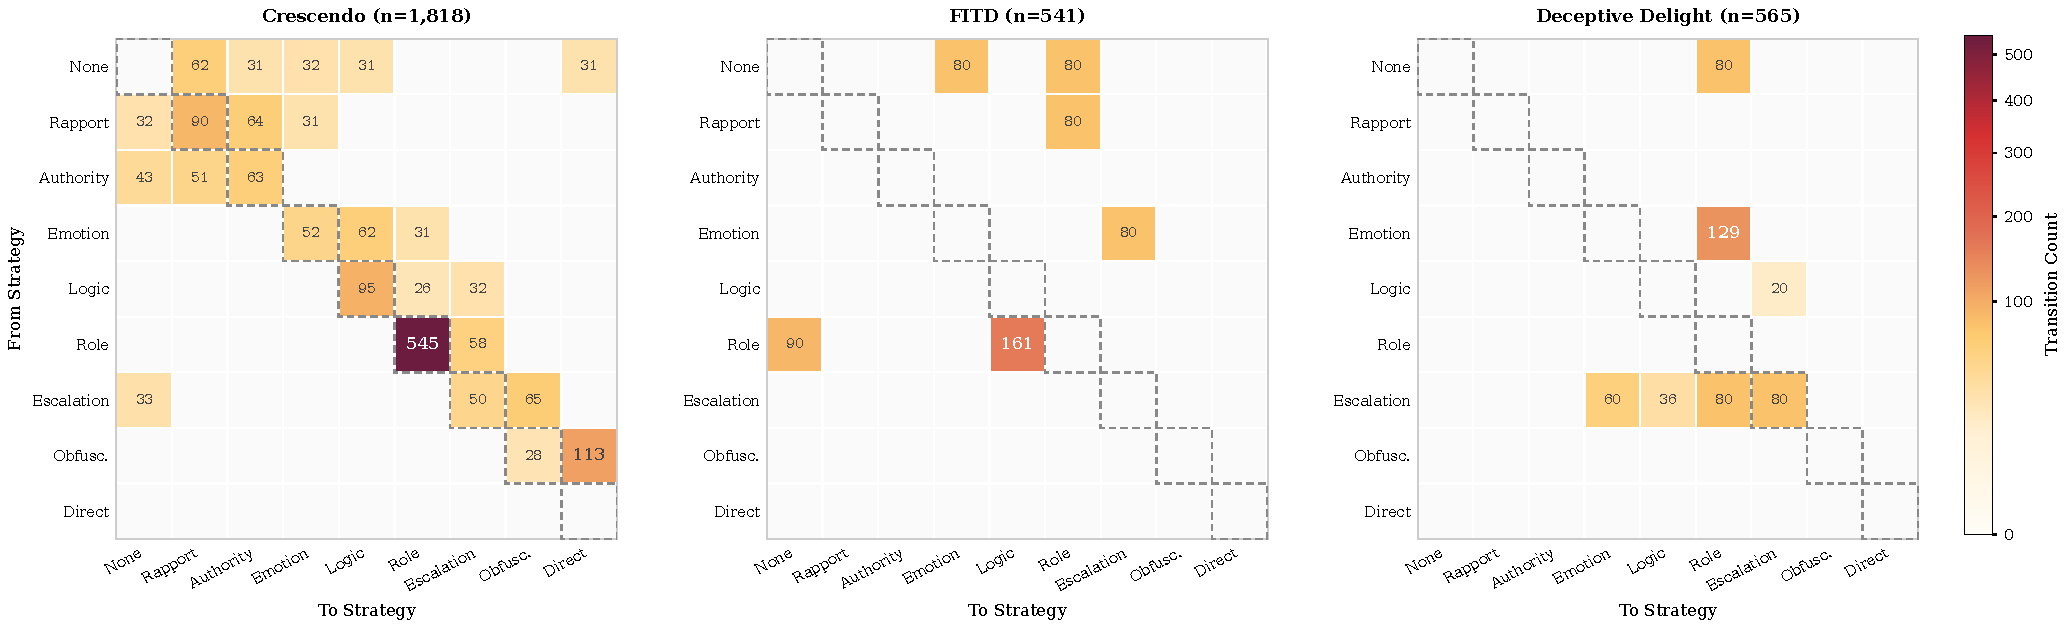
\includegraphics[width=\textwidth]{figures/paper/fig3_strategy_heatmap.pdf}
\caption{Persuasion strategy transition count matrices for three attack families, based on ground-truth intended strategy labels. Strategy labels validated on $n$=50 samples with a single annotator ($\kappa$=0.78); fine-grained trajectory patterns should be interpreted with this limitation. Crescendo exhibits broad coverage across all strategy categories, while FITD and DD concentrate transitions in smaller subsets. Row $i$, column $j$ counts transitions from strategy $i$ at turn $t$ to strategy $j$ at turn $t+1$.}
\label{fig:strategy_heatmap}
\end{figure*}

Figure~\ref{fig:strategy_heatmap} shows transition count matrices for three attack families.
Crescendo conversations exhibit broad transition coverage across all nine strategy categories (1,818 total transitions), with the highest concentration in Role Assignment self-transitions (545); this reflects its gradual escalation design.
FITD conversations show a markedly sparser pattern (541 transitions), with Role$\to$Obfuscation (161) as the dominant transition, consistent with FITD's commitment-consistency exploitation~\citep{cialdini2001influence}.
DD conversations span 5 active source strategies (565 transitions), with Emotion$\to$Obfuscation (129) as the dominant transition, aligning with DD's design of embedding harmful content within emotionally engaging contexts~\citep{deceptivedelight2024}.

\section{Centered CKA Heatmaps}
\label{sec:cka_heatmap}

\begin{figure}[t]
\centering
\includegraphics[width=\columnwidth]{figures/paper/cka_heatmap.pdf}
\caption{Centered CKA similarity~\citep{kornblith2019cka} between encoder variants on IID and OOD data for DeBERTa-v3 and RoBERTa. Low off-diagonal values (vanilla vs.\ adapted variants) confirm that continued pretraining substantially reshapes representations; the MLM vs.\ 9-class block shows distinct geometries (CKA $\leq$ 0.2 on RoBERTa OOD).}
\label{fig:cka_heatmap}
\end{figure}

\section{Embedding Space Visualization}
\label{app:tsne}

Figure~\ref{fig:tsne} visualizes mean-pooled \texttt{[CLS]} embeddings via t-SNE for three representative variants (Vanilla, JB-MLM, 9-Class) on DD OOD and ActorAttack. Vanilla embeddings show dispersed jailbreak clusters with ambiguous decision boundaries, while domain-adapted variants (JB-MLM, 9-Class) produce tighter, more separable clusters. JB-MLM achieves the clearest bimodal separation on both evaluation sets, consistent with its superior detection performance.

\begin{figure}[ht]
\centering
\includegraphics[width=\columnwidth]{figures/paper/embedding_tsne.pdf}
\caption{t-SNE visualization of mean-pooled \texttt{[CLS]} embeddings (perplexity=30) for Vanilla, JB-MLM, and 9-Class variants on DD OOD and ActorAttack (118 samples each; blue=benign, red=jailbreak).}
\label{fig:tsne}
\end{figure}

\section{Cross-LLM Validation}
\label{app:cross_llm}

\begin{table}[ht]
\centering
\footnotesize
\caption{Cross-LLM validation (F1, full conversation). All models are trained on Qwen3-8B data; conditions vary the source of jailbreak (JB) and benign (ben.) conversations at inference. Values are evaluated under a matched 50-sample subset protocol and differ from Table~\ref{tab:evidence_hierarchy}, which uses the full evaluation set.}
\label{tab:cross_llm}
\resizebox{\columnwidth}{!}{%
\begin{tabular}{@{}lcccccc@{}}
\toprule
& \multicolumn{3}{c}{\textit{DD Full}} & \multicolumn{3}{c}{\textit{AA Full}} \\
\cmidrule(lr){2-4} \cmidrule(lr){5-7}
\textbf{Condition} & Van. & MLM & 9-cl. & Van. & MLM & 9-cl. \\
\midrule
Qwen JB + Qwen ben. & .312 & .914 & .997 & .258 & .893 & .972 \\
Llama JB + Llama ben. & .261 & .282 & .433 & .261 & .368 & .321 \\
Llama JB + Qwen ben. & .302 & .778$^{*}$ & 1.000 & .302 & .903 & .801 \\
\bottomrule
\end{tabular}}
\vspace{-2pt}
{\footnotesize $^{*}$High seed variance (std = 0.306): seed 456 outlier (F1 = 0.345); remaining two seeds achieve F1 $\geq$ 0.97.}
\end{table}

Table~\ref{tab:cross_llm} shows three inference conditions. When both jailbreak and benign text come from Llama (row~2), all variants collapse (F1 = 0.26--0.43), but this conflates two sources of distribution shift: unfamiliar jailbreak patterns and unfamiliar benign text. Row~3 isolates jailbreak transferability by pairing Llama jailbreaks with the original Qwen benign distribution. Under this condition, 9-class recovers to F1 = 1.000 on DD and 0.801 on ActorAttack, and JB-MLM reaches 0.903 on ActorAttack. The contrast between rows~2 and~3 shows that the dominant failure mode in row~2 is benign distribution mismatch (false positives from unfamiliar benign text), not inability to recognize cross-LLM jailbreak patterns. Vanilla remains at 0.26--0.31 across all conditions, further confirming that encoders without DAPT lack OOD detection capability regardless of the LLM source. The residual degradation on ActorAttack (0.801 vs.\ 0.972) reflects genuine cross-LLM variation in structurally complex attack patterns.

\begin{table}[ht]
\centering
\footnotesize
\caption{Error decomposition for DD Full cross-LLM conditions (matched 50-sample subsets). TP rate is identical across benign conditions; the F1 collapse in the Llama-only condition (Table~\ref{tab:cross_llm}, row~2) is driven entirely by false positives on unfamiliar benign text.}
\label{tab:cross_llm_error}
\begin{tabular}{@{}lccc@{}}
\toprule
\textbf{Metric} & Van. & MLM & 9-cl. \\
\midrule
TP rate (Llama JB) & 0.0\% & 68.0\% & 100.0\% \\
FP rate (Llama ben.) & 29.3\% & 88.0\% & 90.0\% \\
FP rate (Qwen ben.) & 0.0\% & 0.9\% & 0.0\% \\
\bottomrule
\end{tabular}
\end{table}

Table~\ref{tab:cross_llm_error} decomposes DD Full F1 into true positive and false positive rates. TP rates are identical regardless of the benign source: domain-adapted models detect Llama-generated jailbreaks at the same rate whether evaluated against Qwen or Llama benign text. The F1 collapse in the full Llama condition (Table~\ref{tab:cross_llm}, row~2) is driven entirely by false positives on unfamiliar benign text (FP rate: 88--90\% on Llama vs.\ 0--0.9\% on Qwen for adapted variants). The model implicitly treats non-Qwen text style as a jailbreak indicator, a spurious correlation from single-LLM training data. This failure reflects a data diversity limitation, not a methodological one; mixed-LLM training (Table~\ref{tab:mixed_llm}) partially addresses this confound.

\section{Mixed-LLM Training Results}
\label{app:mixed_llm}

\begin{table}[ht]
\centering
\footnotesize
\caption{Mixed-LLM training (250 Qwen + 250 Llama conversations, 3-seed mean$\pm$std where available). ToxicChat evaluated on balanced set (408 conversations).}
\label{tab:mixed_llm}
\resizebox{\columnwidth}{!}{%
\begin{tabular}{@{}lccccc@{}}
\toprule
\textbf{Variant} & Mixed & DD OOD & AA OOD & FITD OOD & ToxicChat \\
\midrule
9-class & \textbf{.996$\pm$.006} & \textbf{.818$\pm$.096} & \textbf{.504$\pm$.107} & \textbf{.997$\pm$.005} & \textbf{.550$\pm$.052} \\
MLM & .681$\pm$.226 & .289$\pm$.101 & .258$\pm$.075 & .679$\pm$.188 & .256$\pm$.053 \\
Vanilla & .802$\pm$.010 & .291$\pm$.065 & .389$\pm$.073 & .867$\pm$.022 & .356$\pm$.009 \\
\bottomrule
\end{tabular}}
\end{table}

Table~\ref{tab:mixed_llm} reports detection performance when training on a mixed corpus of Qwen3-8B and Llama-3.1-8B conversations. Classification-based DAPT (9-class) maintains the strongest DD OOD performance (0.818$\pm$0.096), outperforming both vanilla (0.291$\pm$0.065) and MLM (0.289$\pm$0.101) by 53\,pp. ActorAttack remains challenging under mixed-LLM conditions (9-class F1\,=\,0.504$\pm$0.107), suggesting structurally complex attacks require larger or more diverse training data. ToxicChat performance shows no significant improvement over single-source training (0.550$\pm$0.052 vs.\ 0.596$\pm$0.087; Section~\ref{sec:human_data}), consistent with ToxicChat being zero-shot single-turn transfer rather than a standard OOD benchmark.

\section{Dataset Scale Validation}
\label{app:scale_validation}

\begin{table}[ht]
\centering
\footnotesize
\caption{Dataset scale validation (1{,}000 Qwen conversations, 3-seed mean$\pm$std). IID results omitted due to train/test overlap (71\% of original test set present in expanded training data).}
\label{tab:scale_validation}
\begin{tabular}{@{}lcc@{}}
\toprule
\textbf{Variant} & DD OOD & AA OOD \\
\midrule
9-class & \textbf{.889$\pm$.041} & \textbf{.913$\pm$.041} \\
MLM & .338$\pm$.010 & .351$\pm$.018 \\
Vanilla & .326$\pm$.000 & .508$\pm$.085 \\
\bottomrule
\end{tabular}
\end{table}

Table~\ref{tab:scale_validation} validates robustness to dataset scale by doubling the training corpus from 500 to 1{,}000 conversations with new topic seeds. The hierarchy 9-class $\gg$ MLM $\approx$ vanilla holds at 2$\times$ scale: classification-based DAPT maintains 40--56\,pp advantage over vanilla, while MLM provides no improvement over vanilla on either attack family (DD: 0.338 vs.\ 0.326; AA: 0.351 vs.\ 0.508).

The performance decline at 1{,}000 conversations may reflect distributional heterogeneity introduced by diverse topic seeds: the additional conversations broaden the training distribution, potentially diluting the concentrated attack-relevant features that smaller, more homogeneous datasets preserve. IID evaluation was precluded by train/test overlap in the expanded dataset (71\%), limiting analysis to OOD metrics. Human-data validation also degrades under scaled training (ToxicChat F1: 0.596 $\to$ 0.341), suggesting the expanded distribution shifts representations away from features useful for both synthetic OOD and human data.

\section{RoBERTa-large DAPT Learning Rate Control}

\begin{table}[ht]
\centering
\footnotesize
\caption{RoBERTa-large (355M) DAPT learning rate control on OOD Full (3-seed mean$\pm$std). Reducing the learning rate worsens both DD and AA, ruling out over-adaptation as the cause of the regression in Table~\ref{tab:cross_encoder}.}
\label{tab:roberta_large_lr}
\begin{tabular}{@{}lcc@{}}
\toprule
\textbf{Config} & DD Full & AA Full \\
\midrule
Vanilla (no DAPT) & .927$\pm$.036 & 1.000$\pm$.000 \\
9-class, LR=$2 \times 10^{-5}$ & .987$\pm$.004 & .946$\pm$.057 \\
9-class, LR=$1 \times 10^{-5}$ & .948$\pm$.034 & .781$\pm$.054 \\
\bottomrule
\end{tabular}
\end{table}

Reducing the DAPT learning rate from $2 \times 10^{-5}$ to $1 \times 10^{-5}$ worsens both DD and AA performance, which rules out over-adaptation as the cause of the regression observed in Table~\ref{tab:cross_encoder}. An MLM-only variant (without classification) produces the same pattern (AA Full = 0.874$\pm$0.014); representation drift from continued pretraining, not classification-specific bias, is the underlying cause. Domain-adaptive fine-tuning narrows the representation space of a sufficiently large encoder and reduces its inherent OOD generalization ability.

\section{TOST Equivalence Sensitivity Analysis}

\begin{table}[ht]
\centering
\footnotesize
\caption{TOST equivalence test (scrambled vs.\ 9-class, $\delta$=5\,pp, 10 seeds). $p < 0.05$ confirms equivalence within $\pm\delta$.}
\label{tab:tost_sensitivity}
\begin{tabular}{@{}lccc@{}}
\toprule
\textbf{Dataset} & $p$ & $d$ & Equivalent? \\
\midrule
DD OOD & $2.06 \times 10^{-9}$ & $-$0.136 & \checkmark \\
FITD OOD & $\approx 0$ & 0.000 & \checkmark \\
ActorAttack & .183 & 0.440 & -- \\
\bottomrule
\end{tabular}
\end{table}

In our 80-sample test set, $\delta = 5$\,pp corresponds to $\approx$4 additional missed attacks. We choose $\delta$\,=\,5\,pp as a conservative threshold; equivalence holds even at $\delta$\,=\,3\,pp on DD ($p < 0.001$, $n$\,=\,10) and FITD ($p \approx 0$). With 10 seeds at $\delta$\,=\,5\,pp, DD and FITD confirm formal equivalence ($p < 10^{-8}$, $|d| \leq 0.14$), demonstrating that label correctness is not a detection factor for template attacks. On ActorAttack, the mean gap is 3.0\,pp with moderate effect size ($d$\,=\,0.44); TOST does not confirm equivalence ($p$\,=\,0.183), indicating that strategy-diverse attacks retain some sensitivity to label quality.

\section{Partition Robustness and Topic Failure Analysis}
\label{app:random_partition}
\label{app:topic_failure}

\subsection{Random Binary Partition Robustness}

\begin{table}[ht]
\centering
\footnotesize
\caption{OOD F1 for 10 random binary partitions of the 9 strategy labels (each partition randomly assigns strategies to group A or B). All partitions use identical Stage-1 DAPT and Stage-2 GRU training; only the binary label mapping differs. Seed 42 (3 runs).}
\label{tab:random_partition}
\resizebox{\columnwidth}{!}{%
\begin{tabular}{@{}lcccc@{}}
\toprule
\textbf{Partition} & \textbf{Group A} & \textbf{IID} & \textbf{DD OOD} & \textbf{AA OOD} \\
\midrule
0 & \{0,2,4,5,7\} & 1.000 & 1.000 & 1.000 \\
1 & \{1,3,5,6,8\} & 1.000 & 1.000 & 1.000 \\
2 & \{0,1,3,7,8\} & 1.000 & 1.000 & 1.000 \\
3 & \{2,4,5,6,7\} & 1.000 & 1.000 & 1.000 \\
4 & \{0,1,2,6,8\} & 1.000 & 1.000 & 1.000 \\
5 & \{0,3,4,7,8\} & 1.000 & 1.000 & 1.000 \\
6 & \{1,2,3,5,6\} & 1.000 & 1.000 & 1.000 \\
7 & \{1,4,6,7\}   & 1.000 & 1.000 & 0.636 \\
8 & \{0,2,3,4,8\} & 1.000 & 1.000 & 1.000 \\
9 & \{0,1,5,7,8\} & 1.000 & 1.000 & 1.000 \\
\midrule
Mean$\pm$Std &  & 1.000$\pm$.000 & 1.000$\pm$.000 & 0.964$\pm$.109 \\
\bottomrule
\end{tabular}}
\end{table}

All 10 partitions achieve perfect IID and DD OOD detection regardless of how the 9 strategy labels are split into two groups. On ActorAttack, 9/10 partitions achieve F1\,=\,1.000; the sole outlier (partition~7, AA F1\,=\,0.636) uses a 4/5 split that isolates a specific strategy cluster. The near-universal success confirms that domain-relevant binary classification---not specific label semantics---drives cross-attack generalization on template attacks. The AA outlier is consistent with the complexity-dependent boundary observed in Section~\ref{sec:decomposition}: structurally complex attacks are sensitive to specific partition choices while template attacks are not.

\subsection{Topic Classification Failure Analysis}

\begin{table}[ht]
\centering
\footnotesize
\caption{Per-turn Fisher ratio (mean across all dimensions) and silhouette score between jailbreak and benign turn embeddings (\texttt{[CLS]} representations). Higher values indicate greater per-turn separability.}
\label{tab:topic_failure}
\begin{tabular}{@{}llcc@{}}
\toprule
\textbf{Model} & \textbf{Dataset} & \textbf{Fisher (mean)} & \textbf{Silhouette} \\
\midrule
Vanilla  & IID test & 0.118 & 0.034 \\
Vanilla  & DD OOD  & 0.401 & 0.411 \\
Vanilla  & AA OOD  & 0.408 & 0.330 \\
\midrule
9-class DAPT & IID test & 0.073 & 0.048 \\
9-class DAPT & DD OOD  & 0.200 & 0.079 \\
9-class DAPT & AA OOD  & 0.832 & 0.301 \\
\midrule
Topic DAPT & IID test & 0.108 & 0.076 \\
Topic DAPT & DD OOD  & 0.653 & 0.274 \\
Topic DAPT & AA OOD  & 0.311 & 0.141 \\
\bottomrule
\end{tabular}
\end{table}

Topic DAPT achieves \emph{higher} per-turn Fisher separability than 9-class DAPT on IID and DD (0.653 vs.\ 0.200 on DD) yet produces far worse conversation-level detection (F1\,=\,0.541 vs.\ 0.994). This rules out per-turn separability destruction as the failure mechanism. The 9-class model instead greatly expands the embedding space (centroid $L_2$ distance 7.5--27.6 vs.\ 0.9--1.1 for vanilla) while distributing both classes broadly, creating richer representation geometry that the downstream GRU exploits over the turn sequence. Topic classification teaches features that separate turns individually but are temporally inconsistent across a conversation---high per-turn separability does not guarantee that the GRU can learn a stable conversation-level decision boundary.

\section{Reproducibility Details}
\label{sec:reproducibility}

\paragraph{Stage-1 training.}
All variants use DeBERTa-v3-base (184M parameters) with learning rate $2 \times 10^{-5}$, AdamW optimizer ($\beta_1$=0.9, $\beta_2$=0.999, weight decay 0.01), linear warmup over the first 10\% of steps, batch size 16, and 4 epochs. MLM variants use 15\% random token masking. Training takes approximately 30 minutes per variant on a single NVIDIA A100 (40GB).

\paragraph{Stage-2 training.}
The BiGRU has hidden dimension 256, 2 layers, and dropout 0.3 (bidirectional, so output dimension 512). The MLP classifier has layers $512 \to 256 \to 2$ with ReLU activation. Training uses learning rate $1 \times 10^{-3}$, Adam optimizer, batch size 32, and 20 epochs with early stopping (patience 5) on validation F1. Stage-2 training completes in under 5 minutes per variant.

\paragraph{Data generation.}
Jailbreak conversations are generated using Qwen3-8B with attack-specific prompt templates. Crescendo conversations follow a 5--8 turn gradual escalation structure. FITD conversations use a 2--3 turn commitment-consistency structure. Deceptive Delight conversations embed harmful content within emotionally engaging 3--5 turn sequences. Benign conversations are generated with topic-anchored prompts across five domains (technology, health, finance, education, general) with matched turn counts.

\paragraph{Strategy annotation.}
Each user turn is annotated by Qwen3-8B using a structured prompt that provides definitions and two examples for each of the nine strategy categories. The prompt instructs the model to output a single category label. All generation and annotation prompts, the full dataset, and training code are available at \url{https://anonymous.4open.science/r/persuasion_turn_jailbreak_detect-C207/}.

\paragraph{Adversarial paraphrasing.}
The paraphrased test set is generated by instructing Qwen3-8B to rephrase each user turn while preserving the communicative intent. The resulting paraphrases have mean BERTScore 0.92 and mean lexical overlap 0.20 with the originals. These metrics confirm substantial surface-level variation.

\paragraph{Cross-checkpoint variance.}
To disentangle Stage-1 from Stage-2 variance, we evaluate three independently trained 9-class DAPT checkpoints (seeds 42, 123, 456) with a fixed downstream BiGRU seed (42). Results: IID F1\,=\,1.000$\pm$0.000, DD OOD\,=\,0.926$\pm$0.026, AA OOD\,=\,0.935$\pm$0.013. Stage-1 training is stable (OOD std\,$\leq$\,2.6\,pp), confirming that the variance reported in the main paper is not dominated by Stage-1 initialization.

\section{End-to-End Fine-Tuning Upper Bound}
\label{app:e2e}

\begin{table}[ht]
\centering
\footnotesize
\caption{Frozen probing vs.\ end-to-end (E2E) fine-tuning for DeBERTa-v3-base 9-class (3-seed mean$\pm$std). E2E unfreezes the Stage-1 encoder during Stage-2 training. Frozen values use main-experiment checkpoints (matching Tables~\ref{tab:main_results}--\ref{tab:evidence_hierarchy}). Table~\ref{tab:frozen_verify} independently verifies these values.}
\label{tab:e2e}
\begin{tabular}{@{}lccc@{}}
\toprule
\textbf{Config} & IID & DD OOD & AA OOD \\
\midrule
Frozen probing & 1.000$\pm$.000 & .997$\pm$.005 & .972$\pm$.026 \\
E2E fine-tuning & 1.000$\pm$.000 & 1.000$\pm$.000 & \textbf{.997$\pm$.005} \\
\midrule
$\Delta$ & .000 & +.003 & +.025 \\
\bottomrule
\end{tabular}
\end{table}

End-to-end fine-tuning unfreezes the Stage-1 encoder during Stage-2 BiGRU training, allowing gradient flow through the full pipeline. On IID and OOD DD, the two configurations are indistinguishable; on structurally complex ActorAttack, E2E recovers +2.5\,pp. The modest gain confirms that frozen probing captures the vast majority of discriminative information encoded by Stage-1 DAPT, and that the remaining OOD gap in the frozen setting reflects downstream optimization constraints rather than missing representational capacity.

\section{Real-World False Positive Rate}
\label{app:wildchat_fpr}

\begin{table}[ht]
\centering
\footnotesize
\caption{False positive rate (\%) on 226 WildChat benign multi-turn conversations (GPT-3.5 users, avg 7.4 turns per conversation). All models trained on synthetic Qwen3-8B data (1{,}000-conversation scale). 3-seed mean$\pm$std.}
\label{tab:wildchat_fpr}
\begin{tabular}{@{}lcccc@{}}
\toprule
\textbf{Variant} & Seed 42 & Seed 123 & Seed 456 & Mean$\pm$Std \\
\midrule
9-class & 66.8 & 61.1 & 76.5 & 68.1$\pm$6.4 \\
MLM & 36.7 & 64.6 & 32.3 & 44.5$\pm$14.3 \\
Vanilla & 47.3 & 42.5 & 54.4 & 48.1$\pm$4.9 \\
\bottomrule
\end{tabular}
\end{table}

Table~\ref{tab:wildchat_fpr} evaluates false positive rates on 226 WildChat benign multi-turn conversations from real GPT-3.5 users (avg 7.4 turns). All variants produce FPR far exceeding deployable thresholds: 9-class is worst at 68.1\%, followed by vanilla (48.1\%) and MLM (44.5\%). Domain adaptation \emph{increases} FPR relative to vanilla (+20\,pp for 9-class), indicating that continued pretraining amplifies dependence on the training benign distribution. This is consistent with the cross-LLM false positive spike (Table~\ref{tab:cross_llm_error}): models trained on synthetic Qwen3-8B benign text implicitly treat unfamiliar conversational styles as jailbreak indicators. High MLM seed variance (std\,=\,14.3\%) suggests that unsupervised pretraining is particularly unstable under benign distribution shift. Deployment requires per-domain benign calibration or mixed-source benign training data.

\paragraph{Post-hoc calibration.}
ROC AUC\,=\,0.700$\pm$0.054 indicates insufficient discrimination between WildChat benign and jailbreak conversations at the representation level. At TPR$\geq$95\%, the optimal threshold still yields FPR\,=\,62.7\%, far above deployable levels. Temperature scaling cannot improve this trade-off, as ROC curves are invariant to monotonic score transforms. The AUC ceiling reflects genuine domain shift: WildChat benign and jailbreak representations overlap substantially, and no post-hoc calibration can overcome this; in-domain benign adaptation is required.

\paragraph{Second benign source: OASST2.}
\label{app:oasst2}

To test whether benign-side shift generalizes beyond WildChat, we evaluate on 200 benign multi-turn conversations from OpenAssistant OASST2~\citep{kopf2023openassistant}---a crowdsourced dataset of real human conversations, distinct from WildChat (GPT-3.5 user logs) in both authorship and topic distribution.

\begin{table}[ht]
\centering
\footnotesize
\caption{OASST2 benign adaptation curve: FPR on 200 OASST2 benign conversations and OOD jailbreak detection F1 as a function of $N$ OASST2 conversations added to training. Seed 42. Compare WildChat (Table~\ref{tab:wildchat_fpr}): FPR reaches 0\% at $N$\,=\,10.}
\label{tab:oasst2_curve}
\begin{tabular}{@{}rccccc@{}}
\toprule
$N$ & FPR (\%) & IID F1 & DD F1 & AA F1 & FITD F1 \\
\midrule
0 & 57.5 & -- & -- & -- & -- \\
10 & 20.5 & 1.000 & 1.000 & 1.000 & 1.000 \\
25 & \textbf{1.5} & 1.000 & 1.000 & 0.953 & 1.000 \\
50 & \textbf{0.5} & 1.000 & 1.000 & 0.990 & 1.000 \\
\bottomrule
\end{tabular}
\end{table}

Baseline FPR on OASST2 (57.5\%) is comparable to WildChat (68.1\%), confirming that benign-side shift is not source-specific but a general consequence of synthetic-only benign training. The adaptation curve follows the same pattern---monotonic FPR reduction with preserved OOD detection---but requires more samples: 25 conversations reduce FPR to 1.5\% (vs.\ 0\% at $N$\,=\,10 for WildChat), and 50 conversations reach 0.5\%. The slower convergence likely reflects greater distributional distance between crowdsourced OASST2 conversations and the synthetic training distribution compared to WildChat's GPT-3.5 user logs.

\subsection{Estimated Dual-OOD Detection Performance}
\label{app:dual_ood}

The OOD detection F1 reported in the main paper evaluates attack-side OOD with IID benign examples (FPR\,=\,0), providing an upper bound. To estimate performance when \emph{both} attack and benign inputs are OOD, we combine per-seed attack recall (from OOD evaluation) with per-seed benign FPR (from WildChat/OASST2 experiments), assuming independence between attack detection and benign false positives. For each seed, we compute binary detection F1 from the resulting TP, FP, FN counts on the OOD test composition (80 jailbreak + 38 benign).

\begin{table}[ht]
\centering
\footnotesize
\caption{Estimated dual-OOD binary detection F1 under different benign conditions (3-seed mean$\pm$std). Attack recall held fixed from OOD evaluation; only benign FPR varies. IID row corresponds to the benign-IID upper bound (FPR\,=\,0).}
\label{tab:dual_ood}
\begin{tabular}{@{}lcc@{}}
\toprule
\textbf{Benign condition} & DD OOD F1 & AA OOD F1 \\
\midrule
IID (FPR\,=\,0) & .994$\pm$.009 & .981$\pm$.019 \\
WildChat, no adapt & .855$\pm$.020 & .842$\pm$.012 \\
OASST2, no adapt & .874$\pm$.009 & .861$\pm$.018 \\
WildChat + 10-shot & .994$\pm$.009 & .981$\pm$.019 \\
OASST2 + 25-shot & .991$\pm$.009 & .978$\pm$.018 \\
\bottomrule
\end{tabular}
\end{table}

Without benign adaptation, dual-OOD F1 drops by 13--14\,pp (DD: $.994 \to .855$; AA: $.981 \to .842$), driven entirely by false positives on OOD benign inputs. After few-shot adaptation---10 WildChat or 25 OASST2 conversations---dual-OOD F1 recovers to within 0.3\,pp of the IID upper bound, confirming that the lightweight adaptation procedure (Section~\ref{sec:benign_shift}) effectively closes the benign distribution gap without compromising attack-side performance.

\section{BERT-base Proxy Baseline}
\label{app:bert_proxy}

\begin{table}[ht]
\centering
\footnotesize
\caption{BERT-base-uncased (110M) frozen probing without DAPT, matching DeepContext's encoder family~\citep{deepcontext2026}. 3-seed mean$\pm$std. DeBERTa-v3 results from Table~\ref{tab:cross_encoder} for comparison.}
\label{tab:bert_proxy}
\resizebox{\columnwidth}{!}{%
\begin{tabular}{@{}lccc@{}}
\toprule
\textbf{Encoder} & IID & DD OOD & AA OOD \\
\midrule
BERT-base (110M), no DAPT & .996$\pm$.006 & .318$\pm$.031 & .275$\pm$.027 \\
DeBERTa-v3 (184M), no DAPT & 1.000$\pm$.000 & .312$\pm$.043 & .258$\pm$.000 \\
DeBERTa-v3 (184M), 9-class & 1.000$\pm$.000 & .994$\pm$.005 & .939$\pm$.047 \\
\bottomrule
\end{tabular}}
\end{table}

Table~\ref{tab:bert_proxy} compares BERT-base-uncased (110M parameters, matching DeepContext's encoder) against DeBERTa-v3-base (184M), both without domain-adaptive pretraining. The two vanilla encoders achieve comparable OOD performance (DD: 0.318 vs.\ 0.312; AA: 0.275 vs.\ 0.258), despite a 1.7$\times$ parameter difference and different pretraining procedures. Both collapse on OOD evaluation while 9-class DAPT recovers to 0.994 (DD) and 0.939 (AA). This confirms that cross-attack generalization is driven by domain adaptation, not encoder architecture or capacity at this scale.

\section{Confidence Calibration}
\label{app:calibration}

\begin{table}[ht]
\centering
\footnotesize
\caption{Expected calibration error (ECE, 10 bins) for 9-class and vanilla on IID and OOD evaluation (3-seed mean$\pm$std). Lower is better.}
\label{tab:calibration}
\begin{tabular}{@{}lccc@{}}
\toprule
\textbf{Variant} & IID & DD OOD & AA OOD \\
\midrule
9-class & $\approx$0.000 & 0.143$\pm$0.053 & 0.116$\pm$0.053 \\
Vanilla & 0.009$\pm$0.007 & 0.669$\pm$0.004 & 0.504$\pm$0.066 \\
\bottomrule
\end{tabular}
\end{table}

The 9-class model achieves substantially lower ECE than vanilla on OOD data (0.12--0.14 vs.\ 0.50--0.67), indicating that domain adaptation improves not only discriminative performance but also confidence calibration. IID calibration is near-perfect for both variants. The residual OOD ECE (0.12--0.14) suggests that temperature scaling could further improve deployment reliability.

\subsection{ToxicChat False Positive Confidence}
\label{app:confidence}

On ToxicChat, 9-class false positives are overwhelmingly high-confidence: 70.2\% of majority-vote FPs exceed $p > 0.9$ (median 0.999), compared to 58.8\% for JB-MLM (median 0.933). Per-seed analysis is more extreme---94--98\% of single-model 9-class FPs are high-confidence (median 1.0), with the borderline fraction (25\%) in majority vote arising from cross-seed disagreement rather than individual model uncertainty. This confirms that the 9-class ToxicChat FPR reflects systematic feature misalignment---classification DAPT shifts benign text into the jailbreak region with high confidence---rather than boundary ambiguity.

\section{Frozen Probing Verification}
\label{app:frozen_verify}

\begin{table}[ht]
\centering
\footnotesize
\caption{Frozen probing vs.\ end-to-end (E2E) fine-tuning (3-seed mean$\pm$std). 9-class: primary DAPT checkpoints; MLM: matched MLM control checkpoints. Frozen probing trains only BiGRU+MLP on frozen DAPT embeddings.}
\label{tab:frozen_verify}
\resizebox{\columnwidth}{!}{%
\begin{tabular}{@{}lcccc@{}}
\toprule
\textbf{Config} & IID & DD OOD & AA OOD & FITD OOD \\
\midrule
Frozen 9-class & 1.000$\pm$.000 & .997$\pm$.005 & .972$\pm$.026 & 1.000$\pm$.000 \\
Frozen MLM & .982$\pm$.016 & .993$\pm$.009 & .941$\pm$.037 & .987$\pm$.009 \\
E2E 9-class & 1.000$\pm$.000 & 1.000$\pm$.000 & .997$\pm$.005 & --- \\
\bottomrule
\end{tabular}}
\end{table}

Table~\ref{tab:frozen_verify} compares frozen probing across DAPT objectives and against end-to-end fine-tuning. On easy OOD (DD, FITD), frozen MLM and frozen 9-class representations perform comparably ($\Delta \leq 1.3$\,pp). On hard OOD (ActorAttack), 9-class retains a modest advantage (0.972 vs.\ 0.941, $\Delta$\,=\,3.1\,pp) with lower variance ($\sigma$\,=\,0.026 vs.\ 0.037). Both far exceed vanilla encoders ($\leq$0.318; Table~\ref{tab:bert_proxy}). The E2E advantage over frozen 9-class is $\leq$2.5\,pp, confirming that Stage-1 representation quality is the primary source of OOD generalization.

A striking asymmetry emerges when comparing frozen probing to the full pipeline (Table~\ref{tab:evidence_hierarchy}): MLM frozen representations \emph{outperform} the full MLM pipeline on AA OOD (0.941 vs.\ 0.893), while 9-class frozen exactly matches its full pipeline (0.972 vs.\ 0.972). This indicates that MLM's cross-seed instability originates in Stage-2 BiGRU training rather than Stage-1 DAPT: the MLM encoder produces adequate representations that are then degraded by unstable downstream optimization. Classification DAPT, by contrast, produces representations that remain robust through Stage-2 training, explaining its consistently lower variance (Table~\ref{tab:evidence_hierarchy}).

This two-level structure (DAPT vs.\ no-DAPT producing a representation quality leap of +70\,pp; classification vs.\ MLM DAPT producing a stability difference) is consistent with two further observations: $\lambda$=0 matches $\lambda > 0$ during E2E fine-tuning (Table~\ref{tab:lambda}), and mean pooling matches BiGRU under E2E (Table~\ref{tab:temporal}). Once DAPT representations are strong, downstream configuration details have minimal impact.

\subsection{Single-Turn Truncation Analysis}
\label{app:truncated}

To isolate whether the ToxicChat evidence-hierarchy reversal (Section~\ref{sec:discussion}) reflects multi-turn structural dependence, we truncate each synthetic test conversation to its last user turn and re-evaluate both 9-class and JB-MLM models (3-seed mean).

\begin{table}[h]
\centering
\caption{Full-conversation vs.\ last-turn-only F1 (3-seed mean). Truncation widens the 9-class advantage, ruling out multi-turn structure as the driver of the ToxicChat reversal.}
\label{tab:truncated}
\begin{tabular}{@{}llcc@{}}
\toprule
\textbf{Dataset} & \textbf{Mode} & \textbf{9-class} & \textbf{JB-MLM} \\
\midrule
IID & Full & 1.000 & .983 \\
IID & Last turn & .991 & .894 \\
\midrule
DD OOD & Full & .997 & .993 \\
DD OOD & Last turn & .942 & .924 \\
\midrule
AA OOD & Full & .972 & .941 \\
AA OOD & Last turn & .978 & .927 \\
\midrule
FITD OOD & Full & 1.000 & .987 \\
FITD OOD & Last turn & 1.000 & .927 \\
\bottomrule
\end{tabular}
\vspace{-2pt}
{\footnotesize Mean $\Delta$ (9-class $-$ MLM): Full +1.6\,pp, Last turn +6.0\,pp. 9-class advantage widens under truncation across all families, indicating the reversal on ToxicChat is driven by distributional differences between synthetic and human text, not by multi-turn structural dependence.}
\end{table}

\paragraph{Representation geometry analysis.}
\label{app:representation}

To characterize the mechanism behind classification DAPT's robustness, we analyze Stage-1 representations across all seven DeBERTa-v3-base variants (seed 42). We extract \texttt{[CLS]} embeddings from 150 test conversations (50 IID + 50 DD OOD + 50 AA OOD) and compute three metrics.

\begin{table}[ht]
\centering
\footnotesize
\caption{Representation geometry and class separability across Stage-1 variants. PR: participation ratio (effective dimensionality of the embedding space). Fisher ratio: inter-class distance$^2$ / sum of intra-class variances. Weight $\Delta$: L2 distance from pretrained weights (relative to pretrained norm).}
\label{tab:representation}
\begin{tabular}{@{}lccc@{}}
\toprule
\textbf{Variant} & \textbf{PR} & \textbf{Fisher} & \textbf{Wt.\ $\Delta$ (\%)} \\
\midrule
Vanilla & 31.9 & $<$0.001 & 0.000 \\
Wiki-MLM & 25.0 & $<$0.001 & 0.221 \\
JB-MLM & 24.6 & $<$0.001 & 0.256 \\
Topic & 14.5 & 0.012 & 0.371 \\
Scrambled & 7.8 & 2.60 & 0.283 \\
9-class & 9.4 & 4.47 & 0.303 \\
Binary & 3.7 & 19.7 & 0.239 \\
\bottomrule
\end{tabular}
\end{table}

Classification variants compress representations into 2--9 effective dimensions (vs.\ 25--32 for MLM/vanilla) while increasing Fisher ratio by 3--5 orders of magnitude. Weight distances from pretrained are comparable across all variants ($\sim$0.2--0.4\%), indicating that the mechanism is representational restructuring rather than parameter-space regularization. Scrambled labels produce similar compression (PR\,=\,7.8, Fisher\,=\,2.6), confirming that the classification objective structure---not label semantics---drives discriminative compression.

\paragraph{Layer-wise localization.}
\label{app:layerwise}

To determine \emph{where} discriminative compression occurs, we compute PR and Fisher ratio at every DeBERTa-v3-base layer (0--12) for four variants (9-class, scrambled, JB-MLM, vanilla) using the same 236-sample evaluation set (seed 42).

\begin{figure}[ht]
\centering
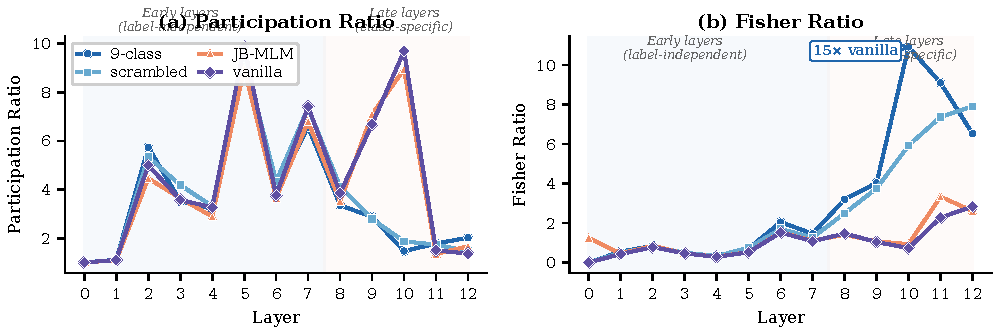
\includegraphics[width=\columnwidth]{figures/paper/fig_layerwise_representation.pdf}
\caption{Layer-wise representation analysis. (a)~Participation ratio: classification variants (9-class, scrambled) show sharp dimensional collapse at layers 9--10 (PR\,$\approx$\,1.5--2.9) while vanilla/JB-MLM maintain high dimensionality (PR\,$\approx$\,7--10). (b)~Fisher ratio (log scale): class separability diverges from layer 8, with 9-class peaking at 10.9 (layer 10) vs.\ vanilla 0.73 (15$\times$).}
\label{fig:layerwise}
\end{figure}

Layers 0--7 show no systematic divergence across variants (Fisher\,$<$\,2.1 for all; PR tracks similar oscillation patterns), consistent with \citet{maennel2020random}'s finding that early layers learn label-independent features. From layer 8 onward, classification-supervised variants diverge sharply: 9-class Fisher rises from 3.2 (layer 8) to 10.9 (layer 10, peak), while vanilla remains below 1.5 throughout. Simultaneously, 9-class PR drops from 3.4 to 1.5 at layer 10---a 6.6$\times$ compression relative to vanilla (PR\,=\,9.7). JB-MLM tracks vanilla across all layers (Fisher\,$\leq$\,3.3, PR\,$\geq$\,1.4), confirming that MLM does not induce discriminative restructuring. Scrambled labels exhibit the same late-layer pattern (Fisher peaks at 7.9, layer 12; PR drops to 1.5, layer 12), reinforcing that any classification signal---regardless of label semantics---triggers late-layer compression.

\paragraph{Discriminative subspace probe.}
\label{app:discriminative_probe}

To test whether the compressed subspace is \emph{sufficient} for OOD detection, we project layer-10 \texttt{[CLS]} representations onto the top-$k$ SVD components and train a logistic regression probe (3 seeds, sklearn default). Controls: random $k$-dimensional projections (10 random bases, mean reported) and vanilla/MLM models under identical projection.

\begin{table}[ht]
\centering
\footnotesize
\caption{Discriminative subspace probe: OOD F1 when projecting layer-10 representations onto top-$k$ SVD components vs.\ random $k$-dimensional projections. 9-class top-3 achieves perfect AA detection with 3/768 dimensions; MLM fails even with all 768.}
\label{tab:discriminative_probe}
\begin{tabular}{@{}llccc@{}}
\toprule
\textbf{Model} & \textbf{Projection} & DD & AA & FITD \\
\midrule
9-class & top-3 & 1.000 & \textbf{1.000} & 1.000 \\
9-class & top-5 & 1.000 & 1.000 & 1.000 \\
9-class & random-3 & 1.000 & 0.928$\pm$.129 & 1.000 \\
9-class & random-5 & 1.000 & 0.952 & 1.000 \\
9-class & full-768 & 1.000 & 1.000 & 1.000 \\
\midrule
scrambled & top-3 & 1.000 & 0.962 & 1.000 \\
scrambled & random-3 & 0.981 & 0.766 & 0.987 \\
\midrule
JB-MLM & top-3 & 1.000 & 0.618 & 1.000 \\
JB-MLM & full-768 & 1.000 & 0.636 & 1.000 \\
JB-MLM & random-5 & 0.685 & 0.584 & 0.744 \\
\bottomrule
\end{tabular}
\end{table}

Three findings establish a link between compression and generalization (Table~\ref{tab:discriminative_probe}). First, 9-class top-3 achieves perfect ActorAttack detection (F1\,=\,1.000) using only 3 of 768 dimensions---all discriminative information resides in the compressed subspace. Second, random 3-dimensional projections degrade to 0.928 on AA, confirming that the specific SVD directions matter. Third, JB-MLM reaches only 0.636 on AA even with all 768 dimensions, demonstrating that without classification-induced compression, the representation lacks the structure needed for cross-attack generalization. DD and FITD are near-ceiling for all models, making ActorAttack the critical test.
SVD directions computed on IID training data only (without OOD test exposure) yield equal or higher F1 than all-data SVD (AA: 0.947 vs.\ 0.904), confirming the subspace is not an artifact of test-set leakage.

\paragraph{SVD necessity ablation.}
\label{app:svd_necessity}

The probe above establishes \emph{sufficiency}: 3 SVD dimensions carry enough information. To test \emph{necessity}, we project \emph{out} the top-3 SVD directions from full 768-dimensional 9-class \texttt{[CLS]} embeddings and re-run BiGRU classification on OOD data (3 seeds). A random-3 removal control verifies that the effect is specific to the discriminative subspace. The top-3 directions explain 89.8\% of training-set variance.

\begin{table}[ht]
\centering
\footnotesize
\caption{SVD necessity ablation: OOD F1 after projecting out top-3 vs.\ random-3 SVD directions from 9-class layer-10 embeddings (3-seed mean$\pm$std).}
\label{tab:svd_necessity}
\resizebox{\columnwidth}{!}{%
\begin{tabular}{@{}lccc@{}}
\toprule
\textbf{Condition} & DD OOD & FITD OOD & AA OOD \\
\midrule
Original 768-dim & 1.000$\pm$.000 & 1.000$\pm$.000 & .994$\pm$.005 \\
Remove top-3 SVD & .831$\pm$.064 & 1.000$\pm$.000 & .938$\pm$.011 \\
Remove random-3 & 1.000$\pm$.000 & 1.000$\pm$.000 & .994$\pm$.005 \\
\bottomrule
\end{tabular}}
\end{table}

Removing top-3 SVD directions degrades DD detection by 17\,pp (F1: $1.0 \to 0.831$) and AA by 5.6\,pp ($0.994 \to 0.938$), while random-3 removal has zero effect. FITD is unaffected by either ablation, indicating its discriminative information is more distributed. Combined with the sufficiency result (Table~\ref{tab:discriminative_probe}), the top-3 SVD directions are both sufficient and necessary for DD detection, sufficient but partially redundant for AA, and sufficient but not necessary for FITD.

\section{Temporal Aggregation Comparison}
\label{app:temporal}

\begin{table}[ht]
\centering
\footnotesize
\caption{Temporal aggregation comparison: mean pooling vs.\ BiGRU under frozen and end-to-end (E2E) settings (3-seed mean$\pm$std). Primary 9-class DAPT checkpoints.}
\label{tab:temporal}
\begin{tabular}{@{}llccc@{}}
\toprule
\textbf{Setting} & \textbf{Aggregator} & DD OOD & AA OOD \\
\midrule
\multirow{2}{*}{Frozen} & BiGRU & .997$\pm$.005 & .972$\pm$.026 \\
& Mean pooling & .991$\pm$.013 & .962$\pm$.015 \\
\midrule
\multirow{2}{*}{E2E} & BiGRU & 1.000$\pm$.000 & .997$\pm$.005 \\
& Mean pooling & 1.000$\pm$.000 & 1.000$\pm$.000 \\
\bottomrule
\end{tabular}
\end{table}

Table~\ref{tab:temporal} compares BiGRU and mean pooling under both frozen and E2E settings. Under frozen probing (the main paper's pipeline), BiGRU provides a marginal advantage on ActorAttack (+1.0\,pp) with overlapping confidence intervals, consistent with the main text finding that temporal order is not a core detection factor ($|\Delta| < 1$\,pp under turn shuffling; Section~\ref{sec:decomposition}). Under E2E fine-tuning, the difference vanishes entirely: mean pooling saturates all benchmarks at F1\,=\,1.000. The choice of frozen BiGRU in the main pipeline reflects a design trade-off: it enables representation-level analysis (CKA, t-SNE) that E2E would confound, while sacrificing $\leq$1\,pp on the hardest OOD set.

\section{Length Stratification Analysis}
\label{app:length}

\begin{table}[ht]
\centering
\footnotesize
\caption{Jailbreak recall by conversation length bin on OOD evaluation (3-seed majority vote). Benign conversations span 12--20 turns; jailbreak conversations span 3--10 turns.}
\label{tab:length}
\begin{tabular}{@{}llccc@{}}
\toprule
\textbf{Dataset} & \textbf{Variant} & 1--3 turns & 4--6 turns & 7--10 turns \\
\midrule
\multirow{2}{*}{DD OOD} & 9-class & --- & 100.0\% & 99.4\% \\
& Vanilla & --- & $\leq$2.6\% & $\leq$1.7\% \\
\midrule
\multirow{2}{*}{AA OOD} & 9-class & 93.3\% & 95.6\% & 100.0\% \\
& Vanilla & 0.0\% & $\leq$2.6\% & 0.0\% \\
\bottomrule
\end{tabular}
\end{table}

Table~\ref{tab:length} stratifies jailbreak recall by conversation length. The 9-class model shows no systematic degradation: ActorAttack recall increases monotonically from 93.3\% (1--3 turns) to 100\% (7--10 turns), and DD recall is near-perfect across all bins.

\paragraph{Length confound.}
Benign conversations (12--20 turns) and jailbreak conversations (3--10 turns) have zero length overlap in the OOD evaluation sets, raising the concern that the model discriminates by conversation length rather than content. Three observations argue against this interpretation:
(1)~Vanilla DeBERTa has access to identical length information via the BiGRU but achieves recall $\leq$2.6\% across all bins; length alone is insufficient without domain-adapted representations.
(2)~At prefix $K$=1, where all conversations are length-equalized, 9-class still achieves F1\,=\,0.773$\pm$0.041 on ActorAttack (Table~\ref{tab:actorattack_full}), demonstrating content-based detection independent of length.
(3)~The model is trained on IID data (Crescendo) and cannot learn OOD-specific length distributions; generalization to unseen length patterns must rely on content features that transfer across attack families.

\paragraph{Direct empirical verification.}
\label{app:length_independence}

\begin{table}[ht]
\centering
\footnotesize
\caption{Turn-count independence verification (9-class DeBERTa-v3-base, same checkpoint as Table~\ref{tab:main_results}, 3 seeds). Evaluated on the full OOD test set (80 jailbreak + 75 benign conversations) rather than the balanced subset used in Table~\ref{tab:main_results}. Part~A: FPR on test benign truncated to $K$ user turns (all seeds FPR\,=\,0). Part~B: WildChat FPR by turn-count bucket (mean$\pm$std). Part~C: jailbreak detection (F1) after padding with benign turns to 15+ total turns (mean$\pm$std where available).}
\label{tab:length_independence}
\resizebox{\columnwidth}{!}{%
\begin{tabular}{@{}llcc@{}}
\toprule
& \textbf{Condition} & \textbf{FPR / F1} & $n$ \\
\midrule
\multicolumn{4}{l}{\textit{Part A: Benign truncation (test set)}} \\[2pt]
& Original (12--20 turns) & FPR = .000 & 38 \\
& Truncated $K$=3 & FPR = .000 & 38 \\
& Truncated $K$=5 & FPR = .000 & 38 \\
& Truncated $K$=8 & FPR = .000 & 38 \\
& Truncated $K$=10$^{*}$ & FPR = .000 & 38 \\
\midrule
\multicolumn{4}{l}{\textit{Part B: WildChat FPR by turn count}} \\[2pt]
& Short (3--10 turns) & FPR = .770$\pm$.105 & 196 \\
& Medium (11--15 turns) & FPR = .942$\pm$.054 & 23 \\
& Long (16+ turns) & FPR = .857$\pm$.117 & 7 \\
\midrule
\multicolumn{4}{l}{\textit{Part C: Jailbreak padding to 15+ turns}} \\[2pt]
& DD original & F1 = .996 & 80 \\
& DD padded & F1 = .971 ($\Delta$=$-$2.5\,pp) & 80 \\
& AA original & F1 = .963 & 80 \\
& AA padded & F1 = .383$\pm$.261 ($\Delta$=$-$57.9\,pp) & 80 \\
\bottomrule
\end{tabular}}
\vspace{-2pt}
{\footnotesize $^{*}$$K$=10 did not truncate any conversation (test benign max $\sim$8 user turns).}
\end{table}

Truncating benign conversations to match jailbreak turn counts (Part~A) produces zero false positives across all truncation levels and all 3 seeds, directly confirming that the model does not use conversation length as a detection shortcut. $K$=3 and $K$=5 are the effective control conditions where all 38 conversations were truncated; $K$=10 exceeds the maximum test benign length and serves as a no-op control.

WildChat FPR by turn count (Part~B) provides complementary evidence: short conversations (3--10 turns, $n$=196) have \emph{lower} FPR than medium-length ones (11--15 turns, $n$=23), inconsistent with a ``short\,=\,jailbreak'' shortcut. Medium and long buckets have limited sample sizes and should be interpreted as directional evidence only.

Padding jailbreak conversations with benign turns (Part~C) reveals an asymmetry: DD detection is resilient ($\Delta$=$-$2.5\,pp), but ActorAttack collapses ($\Delta$=$-$57.9\,pp). Padding experiments append benign turns \emph{after} the complete attack sequence; in practice, adversaries would not dilute their own successful attacks. The collapse nonetheless exposes BiGRU temporal aggregation as vulnerable to attention dilution on subtle attack signals, a limitation discussed in Section~\ref{sec:limitations}.

\section{Inference Efficiency}
\label{app:efficiency}

\begin{table}[ht]
\centering
\footnotesize
\caption{Inference efficiency comparison. DeBERTa+BiGRU and TF-IDF+LR measured on IID test (76 conversations, avg 8.3 turns, single A100). LLM latency from separate OOD evaluation (118 conversations); cross-condition comparison is indicative only.}
\label{tab:efficiency}
\resizebox{\columnwidth}{!}{%
\begin{tabular}{@{}lrcr@{}}
\toprule
\textbf{Method} & Latency (ms) & Params & VRAM \\
\midrule
TF-IDF+LR & 0.43$\pm$0.05 & $\sim$10K & CPU \\
DeBERTa+BiGRU (ours) & 12.1$\pm$1.2 & 186.7M & 862\,MB \\
Qwen3-8B 3-shot$^{\dagger}$ & $\sim$5{,}200 & 8B & $\sim$16\,GB \\
\bottomrule
\end{tabular}}
\vspace{-2pt}
{\footnotesize $^{\dagger}$Qwen3-8B latency from OOD evaluation (DD/AA, 118 conversations); not directly comparable to encoder latency measured on IID test.}
\end{table}

Table~\ref{tab:efficiency} compares inference cost. On matched data (IID test), DeBERTa+BiGRU processes a conversation in 12.1\,ms, 28$\times$ slower than TF-IDF (0.43\,ms), but this speed gap purchases +71\,pp on ActorAttack (F1\,=\,0.972 vs.\ 0.261; Table~\ref{tab:evidence_hierarchy}). LLM-as-judge approaches are orders of magnitude slower ($\sim$5.2\,s per conversation for Qwen3-8B 3-shot) while achieving substantially lower OOD detection (DD\,=\,0.566, AA\,=\,0.652; Table~\ref{tab:llm_judge}). Zero-shot Qwen3-8B achieves F1\,=\,0.0 on DD OOD because it predicts all conversations as benign (Table~\ref{tab:llm_judge}). The full DeBERTa+BiGRU pipeline requires 862\,MB GPU memory, enabling deployment on consumer hardware. The 24.3$\times$ speedup reported in the main text derives from a matched-condition comparison (DisPeD 13.12\,ms vs.\ Qwen3-8B 318.53\,ms on the same GPU and data); the larger gap in Table~\ref{tab:efficiency} reflects different hardware conditions and evaluation sets.

\section{Data Efficiency}
\label{app:data_efficiency}

\begin{table}[ht]
\centering
\footnotesize
\caption{Data efficiency of 9-class DAPT (3-seed mean$\pm$std, sample std with $n{-}1$ divisor) and vanilla baseline (seed 42 only). $N$ = total training conversations (balanced jailbreak/benign).}
\label{tab:data_efficiency}
\begin{tabular}{@{}rlccc@{}}
\toprule
$N$ & \textbf{Variant} & IID & DD OOD & AA OOD \\
\midrule
50 & 9-class & 1.000$\pm$.000 & 1.000$\pm$.000 & .969$\pm$.037 \\
125 & 9-class & 1.000$\pm$.000 & 1.000$\pm$.000 & .975$\pm$.019 \\
250 & 9-class & 1.000$\pm$.000 & 1.000$\pm$.000 & .975$\pm$.035 \\
350 & 9-class & 1.000$\pm$.000 & .978$\pm$.030 & .972$\pm$.033 \\
\midrule
50 & Vanilla & .646 & .529 & .234 \\
125 & Vanilla & .532 & .244 & .244 \\
250 & Vanilla & .987 & .365 & .502 \\
350 & Vanilla & 1.000 & .360 & .489 \\
\bottomrule
\end{tabular}
\end{table}

Table~\ref{tab:data_efficiency} shows that 9-class DAPT reaches near-saturation performance with as few as 50 conversations (25 jailbreak + 25 benign): AA OOD F1\,=\,0.969$\pm$0.037, already surpassing vanilla at full training size ($N$=350, AA\,=\,0.489) by 48\,pp using only 14\% of the data. DD OOD is perfectly solved at all training sizes. Vanilla performance is noisy across $N$ (single seed); the consistent pattern is that vanilla never exceeds DD\,=\,0.53 or AA\,=\,0.50 regardless of training size, while 9-class maintains AA\,$\geq$\,0.969 at all $N$. Seed 456 is systematically lower across all $N$ values, contributing most of the cross-seed variance; this is consistent with the initialization sensitivity observed in the main results.

\section{Auxiliary Loss Weight Ablation}
\label{app:lambda}

\begin{table}[ht]
\centering
\footnotesize
\caption{Effect of auxiliary persuasion loss weight $\lambda$ during Stage-2 E2E fine-tuning (seed 42). Stage-1 DAPT encoder is identical across all rows; only the Stage-2 loss $L = L_{\text{binary}} + \lambda \cdot L_{\text{strategy}}$ varies.}
\label{tab:lambda}
\begin{tabular}{@{}rcccc@{}}
\toprule
$\lambda$ & IID & DD OOD & FITD OOD & AA OOD \\
\midrule
0 & 1.000 & 1.000 & 1.000 & 1.000 \\
0.1 & 1.000 & 1.000 & 1.000 & .990 \\
0.5 & 1.000 & 1.000 & 1.000 & .981 \\
1.0 & 1.000 & 1.000 & 1.000 & .981 \\
2.0 & 1.000 & 1.000 & 1.000 & .944 \\
\bottomrule
\end{tabular}
\end{table}

During Stage-2 E2E fine-tuning, the auxiliary persuasion loss weight $\lambda$ has limited impact on detection (Table~\ref{tab:lambda}): the maximum AA OOD gap across all $\lambda$ values is 5.6\,pp (single seed), comparable to the cross-seed variance ($\sim$6\,pp) observed in the main results. All configurations converge to perfect validation F1 within epoch 1, indicating that DAPT representations already encode sufficient discriminative features for downstream classification (Section~\ref{app:frozen_verify}). The value of persuasion strategy classification lies in Stage-1 DAPT, where it shapes encoder representations that transfer across attack families, not in the Stage-2 auxiliary loss.

\section{OOD Strategy Prediction Analysis}
\label{app:strategy_pred}

\begin{table}[ht]
\centering
\footnotesize
\caption{OOD strategy prediction accuracy (jailbreak turns only) and detection rate for the 9-class model (3-seed mean). $r$: Pearson correlation between per-strategy prediction accuracy and per-strategy detection rate.}
\label{tab:strategy_pred}
\resizebox{\columnwidth}{!}{%
\begin{tabular}{@{}lcccc@{}}
\toprule
\textbf{Dataset} & Strat.\ Acc.\ & Det.\ Rate & Missed (per seed) & $r$ \\
\midrule
DD OOD & 50.1\% & 99.6\% & 0 / 0 / 1 & $\sim$0.45 \\
AA OOD & 50.1\% & 96.2\% & 1 / 7 / 1 & $\sim$0.24 \\
\bottomrule
\end{tabular}}
\end{table}

Table~\ref{tab:strategy_pred} reports OOD strategy prediction accuracy alongside detection rates. Strategy prediction accuracy is substantially above random (50.1\% vs.\ 11.1\% chance for 9 classes) and positively correlated with detection success ($r \approx 0.24$--0.45), but strategy prediction is not the detection mechanism: frozen probing with a randomly initialized strategy head (Appendix~\ref{app:frozen_verify}) achieves 97.2\% AA OOD detection, and $\lambda$=0 (no strategy loss) matches or exceeds $\lambda > 0$ during E2E fine-tuning (Table~\ref{tab:lambda}). The classification objective shapes representations during Stage-1 DAPT training; at inference, strategy predictions are a byproduct of those representations, not a driver of detection.

\section{Cross-Seed Ensemble}
\label{app:ensemble}

\begin{table}[ht]
\centering
\footnotesize
\caption{Majority vote ensemble (3 seeds) vs.\ single-seed mean on OOD Full. ``Fixed'' = samples corrected by ensemble; ``Broke'' = samples corrupted by ensemble.}
\label{tab:ensemble}
\resizebox{\columnwidth}{!}{%
\begin{tabular}{@{}lcccc@{}}
\toprule
\textbf{Variant} & DD single$\to$ens. & AA single$\to$ens. & Fixed & Broke \\
\midrule
9-class & .997$\to$\textbf{1.000} & .972$\to$\textbf{.981} & 5 & 0 \\
MLM & .914$\to$\textbf{1.000} & .897$\to$\textbf{.953} & 26 & 0 \\
Vanilla & .258$\to$.258 & .258$\to$.258 & 0 & 0 \\
\bottomrule
\end{tabular}}
\end{table}

Table~\ref{tab:ensemble} shows that majority vote never corrupts correct predictions (Broke\,=\,0 for all variants). MLM benefits most from ensembling (+8.6\,pp DD, +6.0\,pp AA), because its per-seed errors are complementary: each seed fails on different samples, and the majority corrects these. This further exposes MLM's seed instability: its individual seeds are unreliable, but their errors are uncorrelated. By contrast, 9-class seeds are already highly consistent (std\,$\leq$\,0.026), leaving minimal room for ensemble improvement (+0.3--0.9\,pp). Vanilla errors are systematic (all seeds fail on the same OOD samples), so ensembling provides no benefit.

\subsection{Seed-Level F1 Comparisons}
\label{app:seed_level}

To verify that cross-seed pooling does not mask inconsistent pairwise orderings, Table~\ref{tab:seed_level} reports per-seed F1 for all variants on OOD DD and ActorAttack at full conversation length. The overall evidence hierarchy is maintained across seeds, with 9-class and binary consistently outperforming MLM; scrambled shows one reversal on AA (seed 42).

\begin{table}[h]
\centering
\small
\caption{Per-seed F1 on OOD Full for key variants (seeds 42, 123, 456). The relative ordering is consistent across seeds.}
\label{tab:seed_level}
\resizebox{\columnwidth}{!}{%
\begin{tabular}{@{}lcccccc@{}}
\toprule
& \multicolumn{3}{c}{DD-Full} & \multicolumn{3}{c}{AA-Full} \\
\cmidrule(lr){2-4} \cmidrule(lr){5-7}
\textbf{Variant} & s42 & s123 & s456 & s42 & s123 & s456 \\
\midrule
9-class & 1.000 & 1.000 & .990 & .990 & .935 & .990 \\
Binary & 1.000 & 1.000 & 1.000 & .981 & .990 & 1.000 \\
Scrambled & .990 & 1.000 & 1.000 & .891 & .990 & .971 \\
MLM-only & 1.000 & .990 & .751 & .971 & .925 & .784 \\
Vanilla & .285 & .305 & .348 & .258 & .258 & .258 \\
\bottomrule
\end{tabular}}
\end{table}

\section*{Use of AI Assistance}
We used Claude for coding, code drafting, debugging, and language polishing.
